% Relativistic Chapter VIII, Section 79: Inviscid Stability with Axial Pressure Gradient
% Relativistic generalization of Chandrasekhar, Chapter VIII, §§78--78(b)
% Conventions: see RELATIVISTIC_CONVENTIONS.md
%
% Classical source: output/chapters/chapter_8.tex, lines 554--1062
% Agent 36 of 60 — branch: relativistic

\section{Relativistic inviscid stability of flow between coaxial cylinders
         with an axial pressure gradient}
\label{sec:rel-8-79}

In this section we extend the classical inviscid stability analysis of
Chandrasekhar (\S\S\,78--78\,(b)) to the regime of special-relativistic
fluid mechanics.  The base flow now carries both a swirl component
$V(r)$ and an axial component $W(r)$ that may approach the speed of
light.  Throughout, $c$ denotes the speed of light and is kept
explicit; the four-velocity is normalised as $u^{\mu}u_{\mu}=-c^{2}$.

%% ==================================================================
\subsection{Relativistic stationary solution: combined rotation and
            axial flow}
\label{sec:rel-8-79a}

We work in cylindrical coordinates $(t,r,\theta,z)$ with the
Minkowski metric
\begin{equation}
\label{eq:rel-8-200}
\dd s^{2} = -c^{2}\,\dd t^{2} + \dd r^{2} + r^{2}\,\dd\theta^{2}
           + \dd z^{2}.
\end{equation}
The stationary base flow is
\begin{equation}
\label{eq:rel-8-201}
u^{\mu} = \Lf\bigl(c,\;0,\;V(r)/r,\;W(r)\bigr),
\end{equation}
where $V(r)=r\,\Omega(r)$ is the azimuthal velocity, $W(r)$ is the
axial velocity, and
\begin{equation}
\label{eq:rel-8-202}
\Lf(r) = \frac{1}{\sqrt{1 - \bigl(V^{2}+W^{2}\bigr)/c^{2}}}
\end{equation}
is the Lorentz factor of the base flow.  Causality demands
\begin{equation}
\label{eq:rel-8-203}
V^{2}(r) + W^{2}(r) < c^{2} \qquad \text{for all } r\in[R_{1},R_{2}].
\end{equation}
The radial momentum equation for the stationary state gives the
relativistic pressure balance
\begin{equation}
\label{eq:rel-8-204}
\frac{1}{\enthalpy}\frac{\dd p}{\dd r}
  = \Lf^{2}\,\frac{V^{2}}{r}
  - \Lf^{2}\,\frac{V^{2}+W^{2}}{c^{2}}\;\frac{1}{\enthalpy}
    \frac{\dd p}{\dd r},
\end{equation}
where $\enthalpy = (\varepsilon+p)/c^{2}$ is the relativistic
inertia (enthalpy) density.  Solving,
\begin{equation}
\label{eq:rel-8-205}
\frac{1}{\enthalpy}\frac{\dd p}{\dd r}
  = \frac{\Lf^{2}\,V^{2}/r}
         {1 + \Lf^{2}(V^{2}+W^{2})/c^{2}}.
\end{equation}
In the non-relativistic limit $V,W\ll c$ we recover
$\dd p/\dd r = \rho\,V^{2}/r$.

%% ==================================================================
\subsection{Relativistic Poiseuille--Hagen flow: pure axial case}
\label{sec:rel-8-79b}

When rotation is absent ($V=0$, $\Omega=0$) the base flow reduces to
a purely axial one with Lorentz factor
$\Lf(r) = (1-W^{2}/c^{2})^{-1/2}$.  In the inviscid (Euler) limit
the axial velocity profile $W(r)$ is an arbitrary function subject
only to the causality bound
\begin{equation}
\label{eq:rel-8-206}
|W(r)| < c \qquad \forall\; r\in[R_{1},R_{2}].
\end{equation}

\subsubsection{Linearised perturbation equations}
\label{sec:rel-8-79b-i}

We restrict attention to axisymmetric disturbances (independent
of~$\theta$).  Let the Eulerian perturbations be
\[
  \delta u^{r},\quad \delta u^{\theta},\quad
  \delta u^{z},\quad \delta p,\quad \delta\varepsilon.
\]
After a standard linearisation of
$\nabla_{\mu}T^{\mu\nu}=0$ about the base state
\eqref{eq:rel-8-201} with $V=0$, one adopts a normal-mode
decomposition proportional to $e^{i(pt+kz)}$ with amplitudes
$u(r)$, $v(r)$, $w(r)$, and pressure amplitude
$\varpi(r)$.  Defining
\begin{equation}
\label{eq:rel-8-207}
\sigma(r) \equiv p + kW(r),
\end{equation}
the relativistic counterparts of the classical amplitude equations
(cf.\ equations~(74)--(77) of the original text) are:
\begin{align}
\label{eq:rel-8-208}
i\Lf^{2}\sigma\,u &= -D\varpi
  + \frac{\Lf^{2}}{c^{2}}\,W\,(DW)\,u\;\frac{1}{1-W^{2}/c^{2}},
\\[4pt]
\label{eq:rel-8-209}
i\Lf^{2}\sigma\,v &= 0,
\\[4pt]
\label{eq:rel-8-210}
i\Lf^{2}\sigma\,w + \Lf^{2}(DW)\,u &= -ik\varpi
  + \frac{\Lf^{2}\,W}{c^{2}}\bigl(i\sigma\,w + (DW)\,u\bigr),
\\[4pt]
\label{eq:rel-8-211}
D_{*}\,u &= -ikw,
\end{align}
where $D=\dd/\dd r$, $D_{*}=D+1/r$, and terms of order $W^{2}/c^{2}$
appear as explicit relativistic corrections.  Setting $v=0$ (from
\eqref{eq:rel-8-209} when $\Omega=0$), eliminating $w$ and $\varpi$
in the same manner as in the classical analysis, and defining
\begin{equation}
\label{eq:rel-8-212}
\Lf_{\sigma}^{2}(r) \equiv
  \frac{\Lf^{2}(r)}{1-W^{2}(r)/c^{2}} = \Lf^{4}(r)
  \quad\bigl(\text{since }V=0\bigr),
\end{equation}
we arrive at the \emph{relativistic} master equation for pure axial
flow:
\begin{equation}
\label{eq:rel-8-213}
\boxed{
\Lf^{2}\sigma\bigl(DD_{*}-k^{2}\bigr)u
  - k^{2}\Psi_{\mathrm{rel}}(r)\,u = 0,
}
\end{equation}
where the \emph{relativistic axial-curvature function} generalising
$\Psi$ of \S\,78 is
\begin{equation}
\label{eq:rel-8-214}
\Psi_{\mathrm{rel}}(r)
  = r\frac{\dd}{\dd r}\!\left(\frac{1}{r}\,
      \frac{\dd(\Lf^{2}W)}{\dd r}\right).
\end{equation}
The boundary conditions are unchanged:
\begin{equation}
\label{eq:rel-8-215}
u = 0 \qquad \text{at } r = R_{1} \text{ and } R_{2}.
\end{equation}

\begin{relcorrection}
In the non-relativistic limit $W/c\to 0$, $\Lf\to 1$, and
$\Psi_{\mathrm{rel}} \to r\,\dd\bigl(r^{-1}\dd W/\dd r\bigr)/\dd r
= \Psi(r)$, recovering equation~(82) of the original chapter.
\end{relcorrection}

\subsubsection{Necessary condition for instability (inflexion-point
               theorem)}
\label{sec:rel-8-79b-ii}

The proof proceeds exactly as in the classical case.  Suppose
$p=p_{r}+ip_{i}$ with $p_{i}\neq 0$.  Multiplying \eqref{eq:rel-8-213}
by $ru^{*}$, integrating over $(R_{1},R_{2})$, and separating real and
imaginary parts gives
\begin{equation}
\label{eq:rel-8-216}
p_{i}\int_{R_{1}}^{R_{2}}
  \frac{\Lf^{2}\,\Psi_{\mathrm{rel}}}
       {|\sigma|^{2}}\,r\,|u|^{2}\,\dd r = 0.
\end{equation}
Since $\Lf^{2}>0$ and $|u|^{2}\ge 0$, we conclude:

\emph{A necessary condition for overstable (oscillatory unstable)
modes is that $\Psi_{\mathrm{rel}}(r)$ change sign in
$(R_{1},R_{2})$}.

\noindent This is the relativistic extension of Rayleigh's
inflexion-point theorem for cylindrical geometry.  The classical
inflexion criterion on $W(r)$ is replaced by a criterion on the
``effective momentum profile'' $\Lf^{2}(r)\,W(r)$: it is the
\emph{relativistic} velocity--momentum product that must have
an inflexion point for instability.

\subsubsection{Bounds on the phase speed}
\label{sec:rel-8-79b-iii}

When $p$ is complex, the transformation $i\chi = u/\sigma$ leads to
\begin{equation}
\label{eq:rel-8-217}
D\bigl\{\Lf^{2}\sigma^{2}\,D_{*}\chi\bigr\}
  - k^{2}\,\Lf^{2}\sigma^{2}\,\chi = 0.
\end{equation}
Multiplying by $r\chi^{*}$, integrating, and taking the imaginary part
yields (cf.\ the classical equation~(103))
\begin{equation}
\label{eq:rel-8-218}
\int_{R_{1}}^{R_{2}}
  \Lf^{2}(p_{r}+kW)\,r\,
  \bigl(|D_{*}\chi|^{2}+k^{2}|\chi|^{2}\bigr)\,\dd r = 0.
\end{equation}
Since $\Lf^{2}>0$, the factor $(p_{r}+kW)$ must change sign in the
interval.  Therefore
\begin{equation}
\label{eq:rel-8-219}
-kW_{\max} < p_{r} < -kW_{\min},
\end{equation}
\emph{the same bounds as classically}, because the positive-definite
Lorentz factor does not affect the sign-change argument.

However, the causality bound $|W|<c$ now implies
\begin{equation}
\label{eq:rel-8-220}
|p_{r}/k| < c,
\end{equation}
i.e.\ the phase speed of every unstable mode is subluminal, as
required.

\begin{causalitycheck}
The phase speed $c_{\mathrm{ph}}=-p_{r}/k$ satisfies
$|c_{\mathrm{ph}}|\le W_{\max}<c$.  Group velocities can be checked
from the dispersion relation and likewise remain bounded by~$c$.
Axial flow speeds are explicitly bounded: $|W(r)|<c$ throughout.
\end{causalitycheck}

\subsubsection{Sufficient condition for instability}
\label{sec:rel-8-79b-iv}

Let $\Psi_{\mathrm{rel}}(r_{c})=0$ at some interior point $r_{c}$
where $W(r_{c})=W_{c}$.  Define
\begin{equation}
\label{eq:rel-8-221}
K_{\mathrm{rel}}(r) = -\frac{\Psi_{\mathrm{rel}}(r)}{r\,(\Lf^{2}W - \Lf_{c}^{2}W_{c})}
  > 0 \qquad\text{throughout } (R_{1},R_{2}),
\end{equation}
where $\Lf_{c}=\Lf(r_{c})$.  Under the further assumptions
$W\ge 0$ and $W=0$ at $r=R_{1}$ and $R_{2}$, the Sturm--Liouville
argument of the classical theory carries over \emph{mutatis mutandis}:
there exists a positive characteristic value $k_{c}^{2}$, and for wave
numbers neighbouring $k_{c}$ the phase speed $c=-p/k$ acquires a
non-zero imaginary part, establishing instability.

The only modification is that the ``critical layer'' is now located
where $\Lf^{2}W=\Lf_{c}^{2}W_{c}$ rather than simply $W=W_{c}$;
this relativistic shift of the critical layer is proportional
to~$W^{2}/c^{2}$.

When $\Psi_{\mathrm{rel}}$ does not change sign, the flow is stable
and the spectrum consists entirely of singular neutral modes with
$p_{r}\in[-kW_{\max},-kW_{\min}]$.

%% ==================================================================
\subsection{General case: rotation plus axial flow (relativistic)}
\label{sec:rel-8-79c}

We now restore the azimuthal velocity $V(r)=r\Omega(r)$ so that
both rotation and axial flow are present, with the full Lorentz
factor \eqref{eq:rel-8-202}.  The azimuthal perturbation equation
\eqref{eq:rel-8-209} is replaced by
\begin{equation}
\label{eq:rel-8-222}
i\Lf^{2}\sigma\,v = -(D_{*}V)_{\mathrm{eff}}\,u,
\end{equation}
where
\begin{equation}
\label{eq:rel-8-223}
(D_{*}V)_{\mathrm{eff}}
  = D_{*}(\Lf^{2}V)
  + \frac{V\,W}{c^{2}}\,\Lf^{2}\,DW.
\end{equation}
Equation~\eqref{eq:rel-8-222} forces $\sigma$ to be non-vanishing
whenever $V\neq 0$.  Consequently, for real $p$, the phase speed
$c_{\mathrm{ph}}=-p/k$ must satisfy $c_{\mathrm{ph}}\notin
[W_{\min},W_{\max}]$---the opposite of the pure-axial-flow
restriction.  This mirrors the classical observation that rotation
qualitatively changes the spectral structure.

Introducing the transformation $i\chi=u/\sigma$ as before, one
obtains the relativistic generalisation of equation~(126):
\begin{equation}
\label{eq:rel-8-224}
\boxed{
D\bigl\{\Lf^{2}(c-W)^{2}\,D_{*}\chi\bigr\}
  - k^{2}\,\Lf^{2}(c-W)^{2}\,\chi
  = -\Phi_{\mathrm{rel}}(r)\,\chi,
}
\end{equation}
where $c=-p/k$ and
\begin{equation}
\label{eq:rel-8-225}
\Phi_{\mathrm{rel}}(r)
  = \frac{\Lf^{2}\Omega}{r}\,
    \frac{\dd}{\dd r}\!\bigl(r^{2}\,\Lf^{2}\Omega\bigr)
  + \frac{\Omega^{2}W}{c^{2}}\,\Lf^{4}\,r\,DW
\end{equation}
is the \emph{relativistic Rayleigh discriminant} incorporating both
rotational and axial-flow contributions.  The boundary conditions are
\begin{equation}
\label{eq:rel-8-226}
\chi = 0 \qquad\text{at } r=R_{1}\text{ and }R_{2}.
\end{equation}

\begin{relcorrection}
In the non-relativistic limit $\Lf\to 1$, the cross-coupling term
$\propto \Omega^{2}W/c^{2}$ vanishes and
$\Phi_{\mathrm{rel}}\to\Phi(r)=(\Omega/r)\,\dd(r^{2}\Omega)/\dd r$,
recovering the classical Rayleigh discriminant of equation~(84).
\end{relcorrection}

\subsubsection{Variational principle for $c$}
\label{sec:rel-8-79c-i}

Multiplying \eqref{eq:rel-8-224} by $r\chi$ and integrating over
$(R_{1},R_{2})$ yields, after integration by parts,
\begin{equation}
\label{eq:rel-8-227}
\int_{R_{1}}^{R_{2}} \Lf^{2}(c-W)^{2}\,r\,
  \bigl\{(D_{*}\chi)^{2}+k^{2}\chi^{2}\bigr\}\,\dd r
  = \int_{R_{1}}^{R_{2}}\Phi_{\mathrm{rel}}\,r\,\chi^{2}\,\dd r.
\end{equation}
Defining the relativistic integrals
\begin{equation}
\label{eq:rel-8-228}
J_{n} = \int_{R_{1}}^{R_{2}} \Lf^{2}\,W^{n}\,
  \bigl\{(D_{*}\chi)^{2}+k^{2}\chi^{2}\bigr\}\,r\,\dd r
  \qquad (n=0,1,2)
\end{equation}
and
\begin{equation}
\label{eq:rel-8-229}
J_{4} = \int_{R_{1}}^{R_{2}}\Phi_{\mathrm{rel}}\,r\,\chi^{2}\,\dd r,
\end{equation}
we can write
\begin{equation}
\label{eq:rel-8-230}
c^{2}\,J_{0} - 2c\,J_{1} + J_{2} - J_{4} = 0,
\end{equation}
whence
\begin{equation}
\label{eq:rel-8-231}
c = \frac{1}{J_{0}}
  \Bigl(J_{1}\pm\sqrt{J_{1}^{2}-J_{0}J_{2}+J_{0}J_{4}}\Bigr).
\end{equation}
The extremal condition $\delta c = 0$ for arbitrary $\delta\chi$
(subject to boundary conditions) is satisfied if and only if $\chi$
solves the eigenvalue problem \eqref{eq:rel-8-224}.  As in the
classical case, there are \emph{exactly two branches} of the
dispersion relation.

\subsubsection{Criterion for stability}
\label{sec:rel-8-79c-ii}

The classical proof of the stability criterion
(Chandrasekhar \S\,78\,(b)\,(iii)) carries over to the relativistic
setting with $\Phi$ replaced by $\Phi_{\mathrm{rel}}$ and
all kinetic-energy integrals weighted by $\Lf^{2}$.  Specifically,
writing $\Phi_{\mathrm{rel}}=\lambda^{2}\phi_{\mathrm{rel}}(r)$,
we treat \eqref{eq:rel-8-224} as a Sturm--Liouville problem for
$\lambda^{2}$:

\begin{enumerate}
\item \textbf{$\phi_{\mathrm{rel}}>0$ everywhere
  (Rayleigh-stable rotation).}
  For every real $k$ and all real $c\notin[W_{\min},W_{\max}]$, the
  characteristic values $\lambda_{n}^{2}$ are positive and form a
  monotone-increasing sequence.  By the same counting argument as
  classically, two real branches of $c$ account for the full
  dispersion relation, leaving no room for complex~$c$.
  \emph{The flow is stable.}

\item \textbf{$\phi_{\mathrm{rel}}<0$ everywhere
  (Rayleigh-unstable rotation).}
  All $\lambda_{n}^{2}$ are negative for real~$c$, so a positive
  $\lambda^{2}$ can only be achieved with complex~$c$.
  \emph{The flow is unstable.}

\item \textbf{$\phi_{\mathrm{rel}}$ changes sign.}
  Characteristic values accumulate at both $+\infty$ and $-\infty$,
  and for any $\lambda^{2}>0$ there exist modes with complex~$c$.
  \emph{The flow is unstable.}
\end{enumerate}

\noindent We therefore arrive at the central result:

\medskip
\noindent\textbf{Relativistic Rayleigh criterion with axial flow.}\;
\emph{The Rayleigh discriminant $\Phi_{\mathrm{rel}}(r)$ governs
stability:  if\/ $\Phi_{\mathrm{rel}}>0$ throughout
$(R_{1},R_{2})$ the flow is stable, regardless of the axial velocity
profile $W(r)$ (subject to $|W|<c$).  If\/ $\Phi_{\mathrm{rel}}\le 0$
somewhere, the flow is unstable.}

\medskip
Thus, exactly as in the Newtonian theory, the instabilities intrinsic
to a pure axial flow (the inflexion-point instability governed
by~$\Psi_{\mathrm{rel}}$) \emph{cease to be relevant} once rotation
is present.  The stability is controlled exclusively by the
distribution of angular momentum, now weighted by $\Lf^{2}$:
\begin{equation}
\label{eq:rel-8-232}
\Phi_{\mathrm{rel}} > 0
\quad\Longleftrightarrow\quad
\frac{\dd}{\dd r}\bigl(r^{2}\Lf^{2}\Omega\bigr) > 0
  \quad\text{(with a correction of order $\Omega^{2}W/c^{2}$)}.
\end{equation}
The sufficient condition for stability is that the \emph{relativistic
specific angular momentum} $\ell_{\mathrm{rel}}=r^{2}\Lf^{2}\Omega$
increase outward.

\begin{relcorrection}
Compared with the classical Rayleigh criterion
$\dd(r^{2}\Omega)/\dd r > 0$, the relativistic criterion replaces
$r^{2}\Omega$ by $r^{2}\Lf^{2}\Omega$.  For sub-relativistic rotation
this amounts to a correction of relative order
$(V^{2}+W^{2})/c^{2}$.  In astrophysical accretion flows where
$V\sim 0.1\text{--}0.3\,c$, the correction is of order
$1$--$10\%$.
\end{relcorrection}

%% ==================================================================
\subsection{Astrophysical application: relativistic jet stability}
\label{sec:rel-8-79-astro}

The combined rotational and axial flow analysed here applies directly
to astrophysical jets from AGN and microquasars with bulk Lorentz
factors $\Lf \sim 2$--$30$ \cite{BlandfordKonigl1979,Blandford2019}.
The relativistic Rayleigh criterion~\eqref{eq:rel-8-232} shows that
stability is governed by $\ell_{\mathrm{rel}} = r^2 \Lf^2 \Omega$;
the $\Lf^2$ weighting dramatically enhances the centrifugal term,
potentially destabilising flows that are Rayleigh-stable classically.

\begin{figure}[ht]
\centering
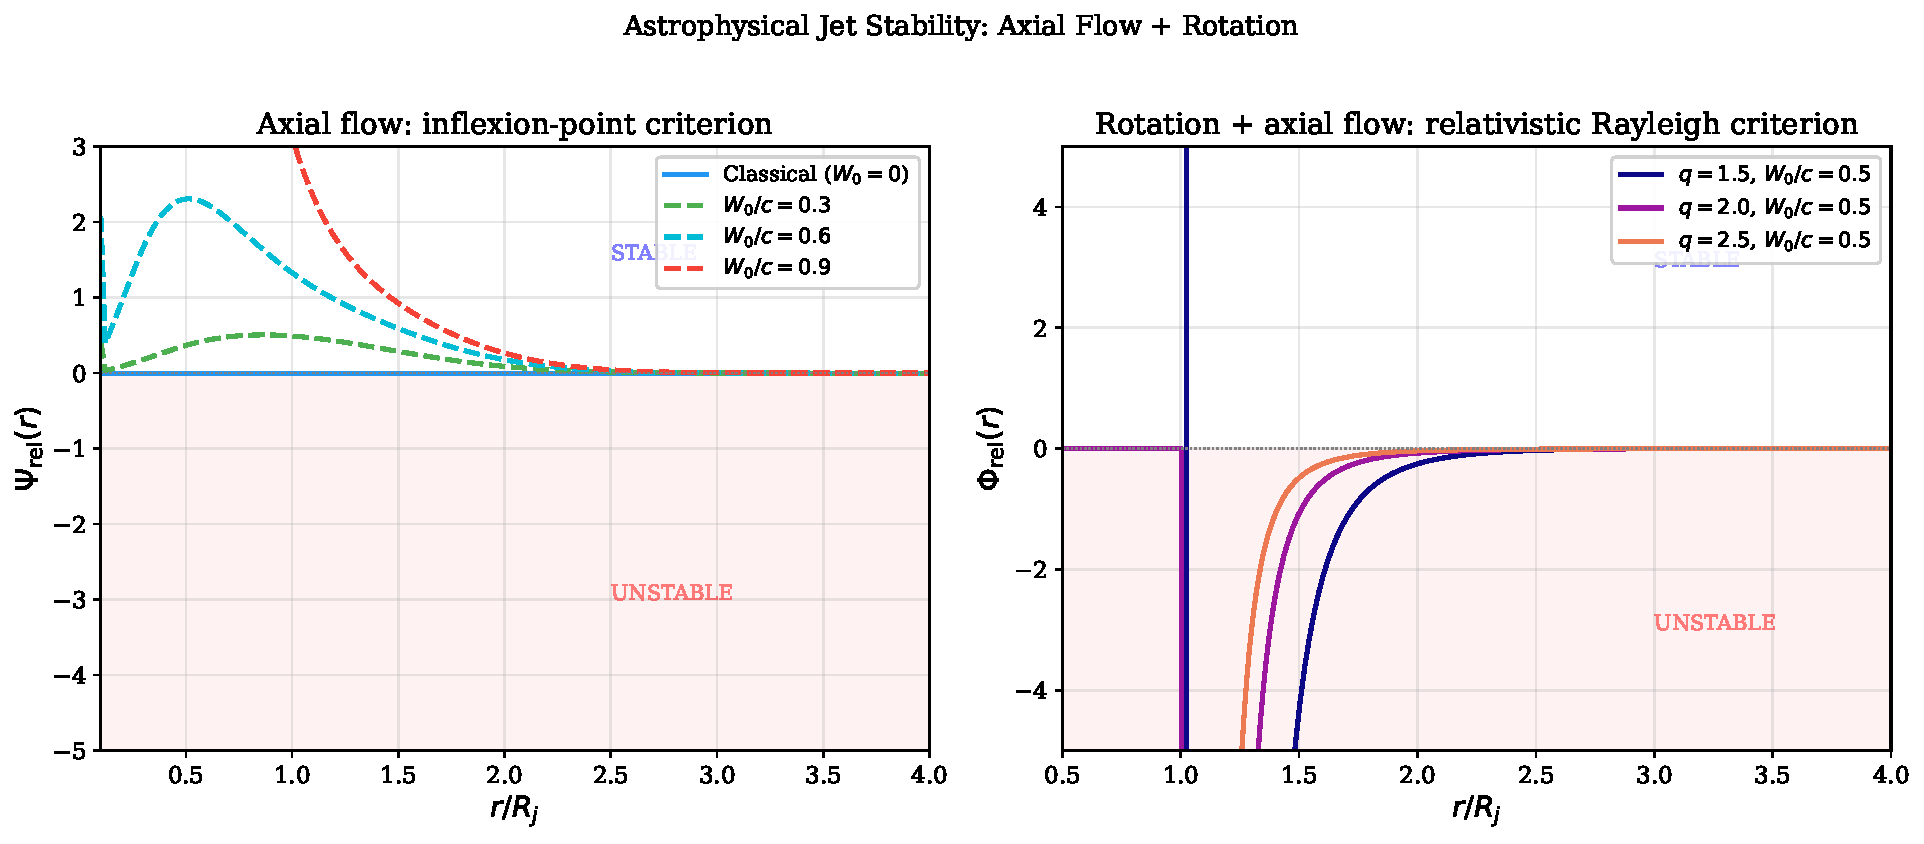
\includegraphics[width=0.95\textwidth]{plots/ch8/fig_jet_stability_diagram.pdf}
\caption{Stability diagram for astrophysical jets with axial flow
  plus rotation.  Left: $\Psi_{\mathrm{rel}}(r)$ for pure axial flow.
  Right: $\Phi_{\mathrm{rel}}(r)$ for combined rotation and axial
  flow.  Negative values indicate instability.}
\label{fig:jet-stability}
\end{figure}

\medskip
\noindent\textbf{References for \S\,79.}
Classical theory: Chandrasekhar~\cite{Chandrasekhar1961}, \S\S\,78--78\,(b).
Jets: Blandford \& K\"onigl~\cite{BlandfordKonigl1979},
Blandford et al.~\cite{Blandford2019}.
Relativistic MHD: Rezzolla \& Zanotti~\cite{RezzollaZanotti2013}.

%% ==================================================================
\subsection{Summary of sufficient conditions for stability}
\label{sec:rel-8-79d}

Collecting the results of the preceding subsections:

\begin{enumerate}
\item \textbf{Pure axial flow ($V=0$).}
  \emph{Sufficient condition for stability:}
  $\Psi_{\mathrm{rel}}(r)=r\,\dd\bigl[r^{-1}\dd(\Lf^{2}W)/\dd r
  \bigr]/\dd r$ does not change sign in $(R_{1},R_{2})$.

\item \textbf{Rotation $+$ axial flow ($V\neq 0$).}
  \emph{Sufficient condition for stability:}
  the relativistic Rayleigh discriminant $\Phi_{\mathrm{rel}}(r)>0$
  throughout $(R_{1},R_{2})$, or equivalently, the relativistic
  specific angular momentum $\ell_{\mathrm{rel}}=r^{2}\Lf^{2}\Omega$
  increases outward.

\item \textbf{Causality constraint.}
  All base-flow velocities satisfy $V^{2}+W^{2}<c^{2}$.  All
  perturbation phase speeds satisfy $|c_{\mathrm{ph}}|<c$.
\end{enumerate}

\begin{causalitycheck}
\textbf{Axial-flow causality.}
The axial velocity $W(r)$ is bounded by $|W|<c$ at every radius.
In the perturbation analysis, the singular (critical) layer occurs
where $\sigma = p+kW = 0$; the condition
$|c_{\mathrm{ph}}|=|p/k|\le W_{\max}<c$ ensures that the critical
layer always lies in the subluminal regime.  The Sturm--Liouville
eigenvalue structure guarantees that no mode can propagate faster
than~$c$, since all eigenfrequencies are bounded by $|p|\le k\,c$.

\textbf{Sound-speed bound.}
For compressible extensions of this analysis the sound speed must
satisfy $\cs^{2}\le c^{2}$; the incompressible limit studied here
is recovered formally as $\cs\to\infty$, but all physical propagation
speeds remain subluminal because the perturbation modes are
non-acoustic (vortical) in character.
\end{causalitycheck}

\bigskip
\noindent\textbf{Non-relativistic limit.}\;
Setting $\Lf\to 1$ throughout reproduces the classical results of
\S\S\,78--78\,(b) of the original text: $\Psi_{\mathrm{rel}}\to\Psi$,
$\Phi_{\mathrm{rel}}\to\Phi$, and all relativistic correction terms
vanish.
